\PassOptionsToClass{aspectratio=169}{beamer}
\documentclass[alsotrans]{beamerswitch}
\usepackage{fprog}

\title{Основни понятия в Haskell}

\date[29.11--6.12.2022 г.]{29 ноември -- 6 декември 2022 г.}

\lstset{language=Haskell,style=Haskell}

\hypersetup{colorlinks,urlcolor=blue,linkcolor=white}

\begin{document}

\begin{frame}
  \titlepage
\end{frame}

\section{Въведение в Haskell}

\begin{frame}
  \frametitle{Какво е Haskell?}

  \pause
  \begin{center}
    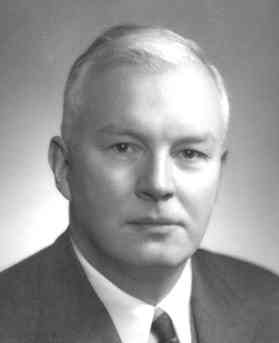
\includegraphics[height=4cm]{images/HaskellBCurry.jpg}\\
    Haskell Brooks Curry\\
    (1900--1982)\\[5ex]
    \imageAttr{Photo of Haskell B. Curry}{Gleb.svechnikov}{https://commons.wikimedia.org/wiki/File:HaskellBCurry.jpg}{CC BY-SA 4.0}
  \end{center}
\end{frame}

\lstset{basicstyle=\small\ttfamily}

\begin{frame}[fragile]
  \frametitle{Какво е Haskell?}

  \pause
\begin{lstlisting}
fact 0 = 1
fact n = n * fact (n-1)
\end{lstlisting}
  \pause
\begin{lstlisting}
quickSort []     = []
quickSort (x:xs) = quickSort less ++ [x] ++ quickSort more
  where less = filter (<=x) xs
        more = filter (>x ) xs
\end{lstlisting}
  \pause
\begin{lstlisting}
@студенти@ = [("@Иван@", 3, 3.5), ("@Мария@", 4, 5.5),
            ("@Петър@", 3, 5.0), ("@Галя@", 2, 4.75)]
@избрани@ = foldr1 (++) [ ' ':@име@ | (@име,курс,оценка@) <- @студенти@,
                                  @оценка@ > 4.5, @курс@ <= 3 ]
\end{lstlisting}
\end{frame}

\lstset{basicstyle=\ttfamily}

\begin{frame}
  \frametitle{Какво е Haskell?}

  \pause
  \begin{itemize}
  \item Чист функционален език (без странични ефекти)
  \item Статично типизиран с автоматичен извод на типовете
  \item Използва нестриктно (лениво) оценяване
  \item Стандартизиран (Haskell 2010 Language Report)
  \end{itemize}
\end{frame}

\begin{frame}
  \frametitle{Помощни материали}

  \begin{enumerate}
  \item S. Thompson. Haskell: The Craft of Functional Programming (2nd ed.). Addison-Wesley, 1999.
  \item P. Hudak, Peterson J., Fasel J. A Gentle Introduction to Haskell 98, 1999 (Internet, 2008).
  \item \href{https://wiki.haskell.org/Haskell}{Haskell Wiki}
  \item \href{https://hackage.haskell.org/}{Hackage} --- централно хранилище с пакети
  \item \href{https://www.haskell.org/ghcup/}{GHCup} --- инсталатор на Haskell
    \begin{itemize}
    \item инсталирайте Haskell Language Server (HLS) за работа с Visual Studio Code
    \item използвайте GHC 9.0.2 вместо актуалната GHC 9.2.x
    \item инсталирайте разширението \href{https://marketplace.visualstudio.com/items?itemName=haskell.haskell}{Haskell} за Visual Studio Code
    \end{itemize}
  \end{enumerate}
\end{frame}

\section{Дефиниции}

\begin{frame}[fragile]
  \frametitle{Синтактични елементи}

  \begin{itemize}[<+->]
  \item Идентификатори: \tt{fact}, \tt{\_myvar}, \tt{студенти}
    \begin{itemize}
    \item имена на обекти, започват с малка буква или \tt\_
    \end{itemize}
  \item Запазени идентификатори: \lst{case}, \lst{if}, \lst{let}, \lst{where}, \ldots
  \item Конструктори: \lst{Integer}, \lst{Maybe}, \lst{Just}, \ldots
    \begin{itemize}
    \item имена на конструкции, започват с главна буква
    \end{itemize}
  \item Числа: \tt{10}, \tt{-5.12}, \tt{3.2e+2}, \tt{1.2E-2}, \tt{0x2f}, \tt{0o35}
  \item Операции: \tt+, \tt*, \tt{\&\%}, \tt{<==>}, \tt{$\spadesuit$}
    \begin{itemize}
    \item поредица от символи (без букви и цифри)
    \item всички операции с изключение на унарния \tt- са инфиксни
    \end{itemize}
  \item Запазени операции: \tt{..} \tt: \tt{::} \tt= \tt\textbackslash \tt| \tt{<-} \tt{->} \tt@ \tt\~ \tt{=>}
  \item Специални знаци: \tt( \tt) \tt, \tt; \tt[ \tt] \tt` \tt\{ \tt\}
  \item Знаци: \lst{'a'}, \lst{'\n'}, \lst{'+'}
  \item Низове: \lst{"Hello, world!"}, \lst{"произволен низ"}
  \end{itemize}
\end{frame}

\begin{frame}
  \frametitle{Декларации и дефиниции}

  \begin{itemize}[<+->]
  \item {}<име> \tta{::} <тип> (типова декларация)
  \item декларира се, че <име> ще се свързва със стойности от <тип>
  \item \alert{типовите декларации са незадължителни: в повечето случаи Haskell може сам да се ориентира за правилния тип}
    \begin{itemize}[<.->]
    \item<+-> \tt{x :: Int}
    \item \tt{y :: Double}
    \item \tt{z :: String}
    \end{itemize}
  \item {}<име> \tta= <израз> (дефиниция)
  \item {}<име> се свърза с <израз>
    \begin{itemize}[<+->]
    \item \lst{x = 2}
    \item \tt{y = \only<+->{fromIntegral }x\^{}2 + 7.5}
    \item \lst{z = "Hello"}
    \item \sta{z = x + y}
    \end{itemize}
  \end{itemize}
\end{frame}

\begin{frame}
  \frametitle{Типове}

  Типовете в Haskell обикновено се задават с конструктори. \pause
  \begin{itemize}[<+->]
  \item \lst{Bool} --- булев тип с константи \lst{True} и \lst{False}
  \item \lst{Char} --- Unicode знаци
  \item Целочислени
    \begin{itemize}
    \item \lst{Int} --- цели числа с фиксирана големина $[-2^{63}; 2^{63}-1]$
    \item \lst{Integer} --- цели числа с произволна големина
    \end{itemize}
  \item С плаваща запетая
    \begin{itemize}
    \item \lst{Float} --- дробни числа с единична точност
    \item \lst{Double} --- дробни числа с двойна точност
    \end{itemize}
  \item Съставни
    \begin{itemize}
    \item \lst{[a]} --- тип списък с \textbf{произволна} дължина и
      елементи от \textbf{фиксиран} тип \tt a
    \item \lst{String = [Char]} --- низ (списък от знаци)
    \item \lst{(a,b,c)} --- тип кортеж (наредена $n$-торка) с
      \textbf{фиксирана} дължина и \textbf{произволни} типове на
      компонентите
    \end{itemize}
  \end{itemize}
\end{frame}

\section{Вградени функции и операции}

\begin{frame}[fragile]
  \frametitle{Стандартен модул \tt{Prelude}}

  \begin{itemize}[<+->]
  \item програмите в Haskell се разделят на модули
  \item \tta{module} <име> \tta{where}
  \item дефинира модул с <име>
  \item \tta{import} <модул> [\tta(<име>\{,<име>\}\tta)]
  \item внася дефинициите <име> от <модул>
  \item ако <име> не е указано, внася всички дефиниции
  \item модулът \lst{Prelude} съдържа набор от често използвани стандартни функции
  \item всички дефиниции от \lst{Prelude} се внасят автоматично във всяка програма
  \end{itemize}
\end{frame}

\begin{frame}
  \frametitle{Стандартни числови функции}

  Аритметични операци

  \tt{+}, \tt{-}, \tt{*}, \tt{/}, \tt{\^{}}, \tt{\^{}\^{}}

  \vspace{2ex}
  Други числови функции

  \lst{div}, \lst{mod}, \lst{max}, \lst{min}, \lst{gcd}, \lst{lcm}

  \vspace{2ex}
  Функции за преобразуване

  \lst{fromIntegral}, \lst{fromInteger}, \lst{toInteger}, \lst{realToFrac}, \lst{fromRational}, \lst{toRational}, \lst{round}, \lst{ceiling}, \lst{floor}

  \vspace{2ex}
  Функции над дробни числа

  \lst{exp}, \lst{log}, \lst{sin}, \lst{cos}, \lst{tan}, \lst{asin}, \lst{acos}, \lst{atan}, \lst{sqrt}, \lst{**}
\end{frame}

\begin{frame}
  \frametitle{Стандартни предикати}

  Числови предикати

  \tt{<}, \tt{>}, \tt{==}, \tt{/=}, \tt{<=}, \tt{>=}, \lst{odd}, \lst{even}

  \vspace{2ex}
  Булеви операции

  \tt{\&\&}, \tt{||}, \lst{not}
\end{frame}

\section{Функции}

\begin{frame}
  \frametitle{Функции в Haskell}

  \begin{itemize}[<+->]
  \item \tt{t1 -> t2} --- тип на функция, която получава параметър от тип \tt{t1} и връща резултат от тип \tt{t2}
  \item {}<име> <параметър> \tta= <тяло>
  \item дефиниция на функция с <име>, един <параметър> и <тяло>
  \item {}<функция> <израз>
  \item прилагане на <функция> над <израз>
    \begin{itemize}[<.->]
    \item \tt{square :: Int -> Int}
    \item \tt{square x = x * x}
    \item \evalsto{square x}4
    \item \evalstoerr{square 2.7}
    \end{itemize}
  \item \alert{Прилагането е с по-висок приоритет от другите операции!}
  \item \evalsto{square 2 + 3}7
  \item \evalsto{square (2 + 3)}{25}
  \end{itemize}
\end{frame}

\begin{frame}
  \frametitle{Функции на повече параметри}
  \begin{itemize}[<+->]
  \item Как можем да изразим двуаргументна функция $f(x,y)$, ако разполагаме само с едноаргументни функции?
  \item Разглеждаме функция $F$ с един аргумент $x$,...
  \item ...която връща като резултат едноаргументната $f_x$,...
  \item ...така че $f_x(y) = f(x,y)$.
  \item Така имаме $f(x,y) = F(x)(y)$.
  \end{itemize}
  \onslide<+->
  \begin{block}{Основна идея}
    Можем да разглеждаме функция с $n+1$ аргумента, като функция с един аргумент, която връща функция с $n$ аргумента.
  \end{block}
  \onslide<+->
  \alert{Това представяне на функциите с повече аргументи се нарича ``къринг'' (``currying'').}
\end{frame}

\begin{frame}[fragile]
  \frametitle{Currying в Haskell}

  \begin{itemize}[<+->]
  \item \tt{t1 \alert{->} (t2 \alert{->} t3)}
    \begin{itemize}
    \item функция с параметър от тип \tt{t1}, която връща функция, която приема параметър от тип \tt{t2} и връща резултат от тип \tt{t3}; или
    \item функция на два параметъра от типове \tt{t1} и \tt{t2}, която връща резултат от тип \tt{t3}
    \end{itemize}
  \item В общия случай: <функция> \tt{\alert{::} t1 \alert{->} (t2 \alert{->}} \ldots \tt{(tn \alert{->} t)}\ldots\tt)
  \item{} <функция> ще очаква $n$ параметъра от типове \tt{t1}, \tt{t2}, \ldots, \tt{tn} и ще връща резултат от тип \tt{t}
  \item{} <функция> <параметър$_1$> \ldots <параметър$_n$> \tta= <тяло>
  \item дефинира <функция> с $n$ параметъра и <тяло>
    \begin{itemize}
    \item \lst{hypothenuse :: Double -> }\alt<+->{\lst{Double -> Double}}{\lst{(Double -> Double)}}
    \item \lst{hypothenuse a b = sqrt (a**2 + b**2)}
    \item \evalstos{\alt<+->{\tt{hypothenuse 3 4}}{\tt{(hypothenuse 3) 4}}}{\tt5}
    \end{itemize}
  \end{itemize}
\end{frame}

\begin{frame}<1-5>

  \frametitle{Частично прилагане на функции}
  Кърингът позволява удобно прилагане на функция към само част от параметрите.
  \begin{itemize}[<+->]
  \item \lst{div50 :: Int -> Int}
  \item \tt{div50\temporal<4>{ x}{ $\!\!\not{\tt x}$}{} = div 50\temporal<4>{ x}{ $\!\!\not{\tt x}$}{}}
  \item \evalsto{div50 4}{12}
  \end{itemize}
\end{frame}

\begin{frame}<1-19>[fragile]
  \frametitle{Функции от по-висок ред}

  \alert{Внимание:} \tt{t1 -> (t2 -> t3)} $\neq$ \tt{(t1 -> t2) -> t3}!\pause
  \begin{itemize}[<+->]
  \item операцията \tt{->} е \textbf{дясноасоциативна}
  \item \tt{t1 -> (t2 -> t3)} $\equiv$ \tt{t1 -> t2 -> t3}
  \item \tt{(t1 -> t2) -> t3} --- функция, която връща резултат от тип \tt{t3}, а приема като единствен параметър функция, която приема един параметър от тип \tt{t1} и връща резултат от тип \tt{t2}
  \item \alert{функция от втори ред}
    \begin{itemize}
    \item \lst{twice f x = f (f x)}
    \item \lst{twice :: }\alt<-11>{\lst{(Int -> Int) -> Int -> Int}}{\lst{(t -> t) -> t -> t}}
    \item \evalstop{twice square 3}{81}
    \item \evalstop{twice (mod 13) 5}1\pause
    \item \lst{diag f x = f x x}
    \item \lst{diag :: }\alt<-18>{\lst{(Int -> Int -> Int) -> Int -> Int}}{\lst{(t1 -> t1 -> t) -> t1 -> t}}
    \item \evalstop{diag div 5}1
    \item \evalstop{diag hypothenuse 1}{1.4142135623730951}
    \end{itemize}
  \end{itemize}
\end{frame}

\begin{frame}
  \frametitle{Функции и операции}
  \begin{itemize}[<+->]
  \item Функциите в Haskell са винаги с \textbf{префиксен} запис
  \item Операциите в Haskell са винаги \textbf{бинарни с инфиксен}
    запис.
    \begin{itemize}
    \item \alert{Изключение:} унарен минус: \tt{-a}
    \item \evalstoerr{square -x}
    \item \evalsto{square (-x)}4
    \end{itemize}
  \item Преобразуване на двуаргументни функции към бинарни операции: \tta`<функция>\tta`
    \begin{itemize}
    \item \evalsto{13 `div` 5}3
    \item \evalstoerr{2 `square`}
    \end{itemize}
  \end{itemize}
\end{frame}

\begin{frame}
  \frametitle{Операции и функции}
  \begin{itemize}[<+->]
  \item Преобразуване на операции към двуаргументни функции: \tta(<операция>\tta)
    \begin{itemize}
    \item \evalsto{(+) 2 3}5
    \item \lst{plus1 = (+) 1}
    \item \lst{square = diag (*)}
    \end{itemize}
  \item Преобразуване на операции към едноаргументни функции (отсичане на операции)
    \begin{itemize}
    \item \tta(<израз> <операция>\tta) --- ляво отсичане
    \item \tta(<операция> <израз>\tta) --- дясно отсичане
    \item \evalstop{(2\^) 3}8
    \item \evalstop{(\^2) 3}9
    \item \lst{square = (\^2)}
    \item \evalstoerrp{(-5) 8}
    \item \evalstop{twice (*2) 5}{20}
    \item \lst{positive = (>0)}
    \item \lst{lastDigit = (`mod` 10)}
    \end{itemize}
  \end{itemize}
\end{frame}

\begin{frame}
  \frametitle{\tt{if} \ldots \tt{then} \ldots \tt{else}}
  \begin{itemize}[<+->]
  \item \tta{if} <условие> \tta{then} <израз$_1$> \tta{else} <израз$_2$>
    \begin{itemize}[<.->]
    \item Ако <условие> е \lst{True}, връща <израз$_1$>
    \item Ако <условие> е \lst{False}, връща <израз$_2$>
    \end{itemize}
  \item \lst{abs x = if x < 0 then -x else x}
  \item \lst{fact n = if n == 0 then 1 else n * fact (n - 1)}
  \item \evalstoerr{if x > 5 then x + 2 else "Error"}
  \item \alert{<израз$_1$> и <израз$_2$> трябва да са от един и същи тип!}
  \item \alert{<условие> трябва да е от тип \tt{Bool}!}
  \end{itemize}
\end{frame}

\end{document}
